\section{Methods}
%describe the methods, the data, the assumptions, the scenarios, a brief few 
%sentences on Temoa itself.
This work collected data from multiple sources to populate a model of the 
Illinois electric grid. This simulated representation of the state of 
Illinois relies on the Temoa framework, an open source tool built by the North 
Carolina State University that enables energy system optimization and 
techno-economic analysis 
\cite{decarolis_temoa_2010,decarolis_modelling_2016,decarolis_formalizing_2017}.

\subsection{Optimization Analysis}
This work established optimal solutions to 
various scenarios which illuminate the potential impact of nuclear plant 
closures and other policy options on the cost of power in Illinois. These 
simulations  also explore the state of Illinois' ability to meet its aggressive 
carbon goals with and without maintenance and expansion of nuclear power 
capacity. 

\begin{align}
\intertext{minimize} 
&\sum_{g=1}^G\int_{t=2030}^{t=2050} c_g(t)x_g(t)\\
\intertext{subject to}
& \sum_{j=1}^m cf_j P_j x_j(t) \ge D(t),& j 1,...,m\\
\sum_{g=0}^G \epsilon P_j x_j(t) &\ge D(t),& j 1,...,m\\
\intertext{where}
G&=\text{number of generators}&\\
\end{align}


Assumptions and constraints in these simulations differentiate the scenarios 
presented here. Each optimized scenario is the solution to a linear programming 
problem  comprised of two key components. First, the objective function in this case 
minimizes the total system cost of the energy grid in the state of Illinois. 
Second, a set of constraints limit the model soluations. Then, optimization 
proceeds by varying all free parameters within the scope of the defined constraints in order to meet the objective.

In this case, Temoa varies the deployed ratio of generation technologies on the 
Illinois electric grid, within the constraints of various policies, to minimize 
cost. The simulations each begin in the year 2020 
and proceed through 2050. The initial condition in 2020 represents the current 
electricity generation mix in the state of Illinois today.

\FloatBarrier
\subsection{Data}
% paragraph on data sources
Data sources for this model of Illinois included multiple national and regional 
databases. Primarily this work relied on federal and international databases from the 
Energy Information Administration 
\cite{us_energy_information_administration_eia_preliminary_2021,energy_information_administration_state_2020,us_energy_information_administration_eia_electric_2021,us_energy_information_administration_eia_illinois_2020}, 
the U.S. Geological Survey \cite{hoen_united_2018}, 
International Energy Agency \cite{lorenczik_projected_2020}, 
the Nuclear Energy Agency \cite{crozat_full_2018}
, the Nuclear Regulatory Commission \cite{united_states_nuclear_regulatory_commission_illinois_2020}, 
the Intergovernmental Panel on Climate Change 
\cite{intergovernmental_panel_on_climate_change_annex_2014,intergovernmental_panel_on_climate_change_climate_2014,intergovernmental_panel_on_climate_change_climate_2014-1,intergovernmental_panel_on_climate_change_climate_2014-2}
the Interstate Renewable Energy Council 
\cite{sherwood_us_2009,sherwood_us_2010,sherwood_us_2011,brown_solid_1996,sherwood_us_2012,sherwood_us_2013,sherwood_us_2014}
and the Department of Energy's EERE and NE offices 
\cite{us_department_of_energy_capital_2016}, the National Renewable Energy 
Laboratory \cite{nrel_national_renewable_energy_laboratory_2020_2020}.
Industry sources included the World Nuclear Association
\cite{world_nuclear_association_nuclear_2017}
, 
the Nuclear Energy Institute 
\cite{desai_nuclear_2018,desai_nuclear_2020,murphy_impacts_2019,tessum_air_2019},
Rockland Capital Generation \cite{rockland_capital_natural_2021},
Sargent \& Lundy \cite{sargent__lundy_capital_2020}, 
Lazard \cite{ray_lazards_2020},
and others 
\cite{the_solar_foundation_national_2020,solar_energy_industries_association_illinois_2020,rutovitz_calculating_2015}.


% paragraph on reproducibility and location of data/analysis
This work was conducted in the open under a BSD-3 open-source license by the 
Advanced Reactors and Fuel Cycles group at the University of Illinois. The 
data, models, and assumptions used in his work can all be found and explored at 
open source repository at 
\href{https://github.com/arfc/2021-04-nm-illinois}{github.com/arfc/2021-04-nm-illinois}.

\FloatBarrier
\section{Scenarios Simulated}\label{sec:simulations}

This model of Illinois' electric generation leverages robust data and populates 
an open-source framework for simulating and optimizing energy systems, 
the Temoa framework (Tools for Energy Model Optimization and Analysis). 


\begin{wrapfigure}{l}{0.3\linewidth}
\begin{center}
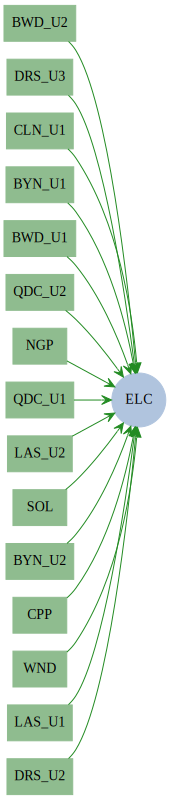
\includegraphics[height=0.5\textheight]{../data/bau_illinois_input_graphviz/bau_illinois.png}
\end{center}
\caption{The directed graph, implemented in Temoa, representing the electric grid in Illinois.}
\label{fig:temoa_graph}
\end{wrapfigure}

In each scenario, the solution gives the energy generation mix, $x_g$,
for the Illinois electric grid to minimize system cost while meeting system
constraints (zero carbon by 2030, optimistic renewable energy and energy
storage deployment speeds, land availability limitations, etc.)
All begin with the same initial condition and. The following parameters and limits are varied to distinguish there

This report will describe the results of the scenarios described in Table \ref{tab:scenarios}. 
There are twelve, in three major categories. First, the steady demand cases SD1-6 include one business as usual case and five cases exploring the impact of carbon limits and premature nuclear energy closure on the minimum achievable cost. These simulations make conservative assumptions about the cost and availability of advanced nuclear power. To explore the importance of these assumptions, two additonal classes of simulations were explored. In the XN (expensive nuclear) cases, advanced nuclear reactors are assumed to be twice as expensive to build than is currently expected. In the ZN (zero advanced nuclear) cases, advanced nuclear power is not available in time to contribute to carbon reductions in Illinois before 2050.  

\section{
Basic constraints;
In SDx and XNx

Utility scale solar is restricted to 10 GW by 2030, reflecting an aggressive and optimistic build out based on CEJA goals.
Wind turbines are restricted to 13.8 GW by 2030, reflecting an aggressive and optimistic build out based on CEJA goals.
Residential solar is allowed to increase at a steady rate, but is capped at 75% of the technical resource availability, determined from a GIS analysis by NREL (i.e. 75% of the theoretical limit).
In ZNx

The constraints on utility scale wind and solar are lifted. It is not possible to achieve zero carbon without advanced nuclear under the above constraints.
Key observations:

Increasing the investment cost for advanced nuclear by 200% has an almost negligible impact on total system cost.
Zero advanced nuclear scenarios are technically less costly, but require an unimaginably aggressive build of solar by 2030 (56 GW!!)
Zero advanced nuclear scenarios require about 12% land use change for renewables (4% land area for rooftop solar). Keeping the nuclear plants open through 2050 halves this requirement (since nuclear is half of IL generation, currently).
Keeping the nuclear plants open through 2050 would reduce e-waste by 600,000 metric tons. Using advanced nuclear saves about 900,000 metric tons.
Keeping the nuclear plants open through 2050 avoids 25 million metric tons of lifecycle CO2 emissions if advanced nuclear is used, and 30 million metric tons if majority renewables is used. Pursuing advanced nuclear over renewables saves about 5 million metric tons.
